% !TEX TS-program = pdflatex
% !TEX encoding = UTF-8 Unicode

% This is a simple template for a LaTeX document using the "article" class.
% See "book", "report", "letter" for other types of document.

\documentclass[11pt]{article} % use larger type; default would be 10pt

\usepackage{amsmath}
\usepackage{amsfonts}
\usepackage[utf8]{inputenc} % set input encoding (not needed with XeLaTeX)

%%% Examples of Article customizations
% These packages are optional, depending whether you want the features they provide.
% See the LaTeX Companion or other references for full information.

%%% PAGE DIMENSIONS
\usepackage{geometry} % to change the page dimensions
\geometry{letterpaper} % or letterpaper (US) or a5paper or....
\geometry{margin=1in} % for example, change the margins to 2 inches all round
% \geometry{landscape} % set up the page for landscape
%   read geometry.pdf for detailed page layout information

\usepackage{graphicx} % support the \includegraphics command and options

% \usepackage[parfill]{parskip} % Activate to begin paragraphs with an empty line rather than an indent

%%% PACKAGES
\usepackage{booktabs} % for much better looking tables
\usepackage{array} % for better arrays (eg matrices) in maths
\usepackage{paralist} % very flexible & customisable lists (eg. enumerate/itemize, etc.)
\usepackage{verbatim} % adds environment for commenting out blocks of text & for better verbatim
\usepackage{subfig} % make it possible to include more than one captioned figure/table in a single float
\usepackage{layout} % see margins
\usepackage{kbordermatrix} % pretty matrices (use $\kbordermatrix{...}$)
\usepackage{hyperref} % for links
\usepackage{mathds} % for fancy E, Z, H, etc

\usepackage{listings} % code blocks (use \begin{lstlisting} and \end{lstlisting})
\usepackage[T1]{fontenc} % get straight double quotes in listings code blocks
\lstset{ % get nice tildes in listings code blocks
    literate={~} {$\sim$}{1}
}
% These packages are all incorporated in the memoir class to one degree or another...

\usepackage[nodayofweek,level]{datetime}
%%% HEADERS & FOOTERS
\usepackage{fancyhdr} % This should be set AFTER setting up the page geometry
\setlength\parindent{24pt}
%%% END Article customizations

\title{\textbf{Math 189: Case Study 4}\\Calibrating a Snow Gauge}
\author{Sherry Diep, Sandra Hui, David Lee, Irving Valles, Albert Xu, Mark Yee}
\date{March 10, 2016}

\begin{document}
\maketitle

\section*{Introduction}
Despite the many advancements of our modern day society, many if not all of communities continue to face the inconveniences of natural disasters. Some of these natural disasters remain unpredictable, but researchers still progressively attempt to find means to create more accurate predictors for communities to prepare properly.

One versatile invention that has been in use is the snow gauge. This equipment works similar to a rain gauge, but rather than measure the precipitation of liquids, the snow gauge measures solid precipitation (Bergman, 1982). Application of this snow gauge includes understanding the way avalanches function. These reports identify avalanches derived from either small loose-snow avalanches or much larger slab avalanches, which depends on how the snow is packed (Armstrong, 1976). Other hazards snow gauges are used for is in flooding settings. In these situations, raining in areas where there is snow is quite hazardous as how the snow is packed affects how much rain is contained and how much is not (Kattelmann, McGurk, Berg, Bergman, Baldwin, \& Hannaford, 1983). Differences found in measurements from this gauge will provide valuable information on the condition of snow and risks for flood in rainy circumstances.

In particular, the data set we are looking at is derived from a gamma transmission gauge, which operates through photon collection of a radioactive source. However, accuracy of this snow gauge may be reduced over time. Because the gamma transmission gauge relies on a radioactive source, radioactive decay may occur and generate inaccurate measurements (Bergman, 1982). The following analysis focuses on the calibration of the snow gauge.

\section*{Fitting}
Our data came from a calibration of USDA Forest Service snow gauges in the Sierra Nevada mountains near Soda Springs, California. We were provided a total of 90 data points generated from 9 different polyethylene blocks, each simulating a different quantity of snow. For each block, a total of 30 gauge measurements were recorded, and the greatest and least one third were thrown out. The remaining 10 samples for each block were used in our data set. The units of density were grams per cubic centimeter, and the reported gain indicated the gamma photon count by the gauge’s detector. The density of the snowpack typically ranges from 0.1 to $0.6 g/cm^3$. To simulate this, our most dense polyethylene block had a density of $0.686 g/cm^3$, while the least dense block was just $0.0010 g/cm^3$.

Rather than directly use all 90 data points, we first performed a linear regression on the average of the log transformed gain values for each polyethylene block density. The regression plot is shown below.
\begin{center}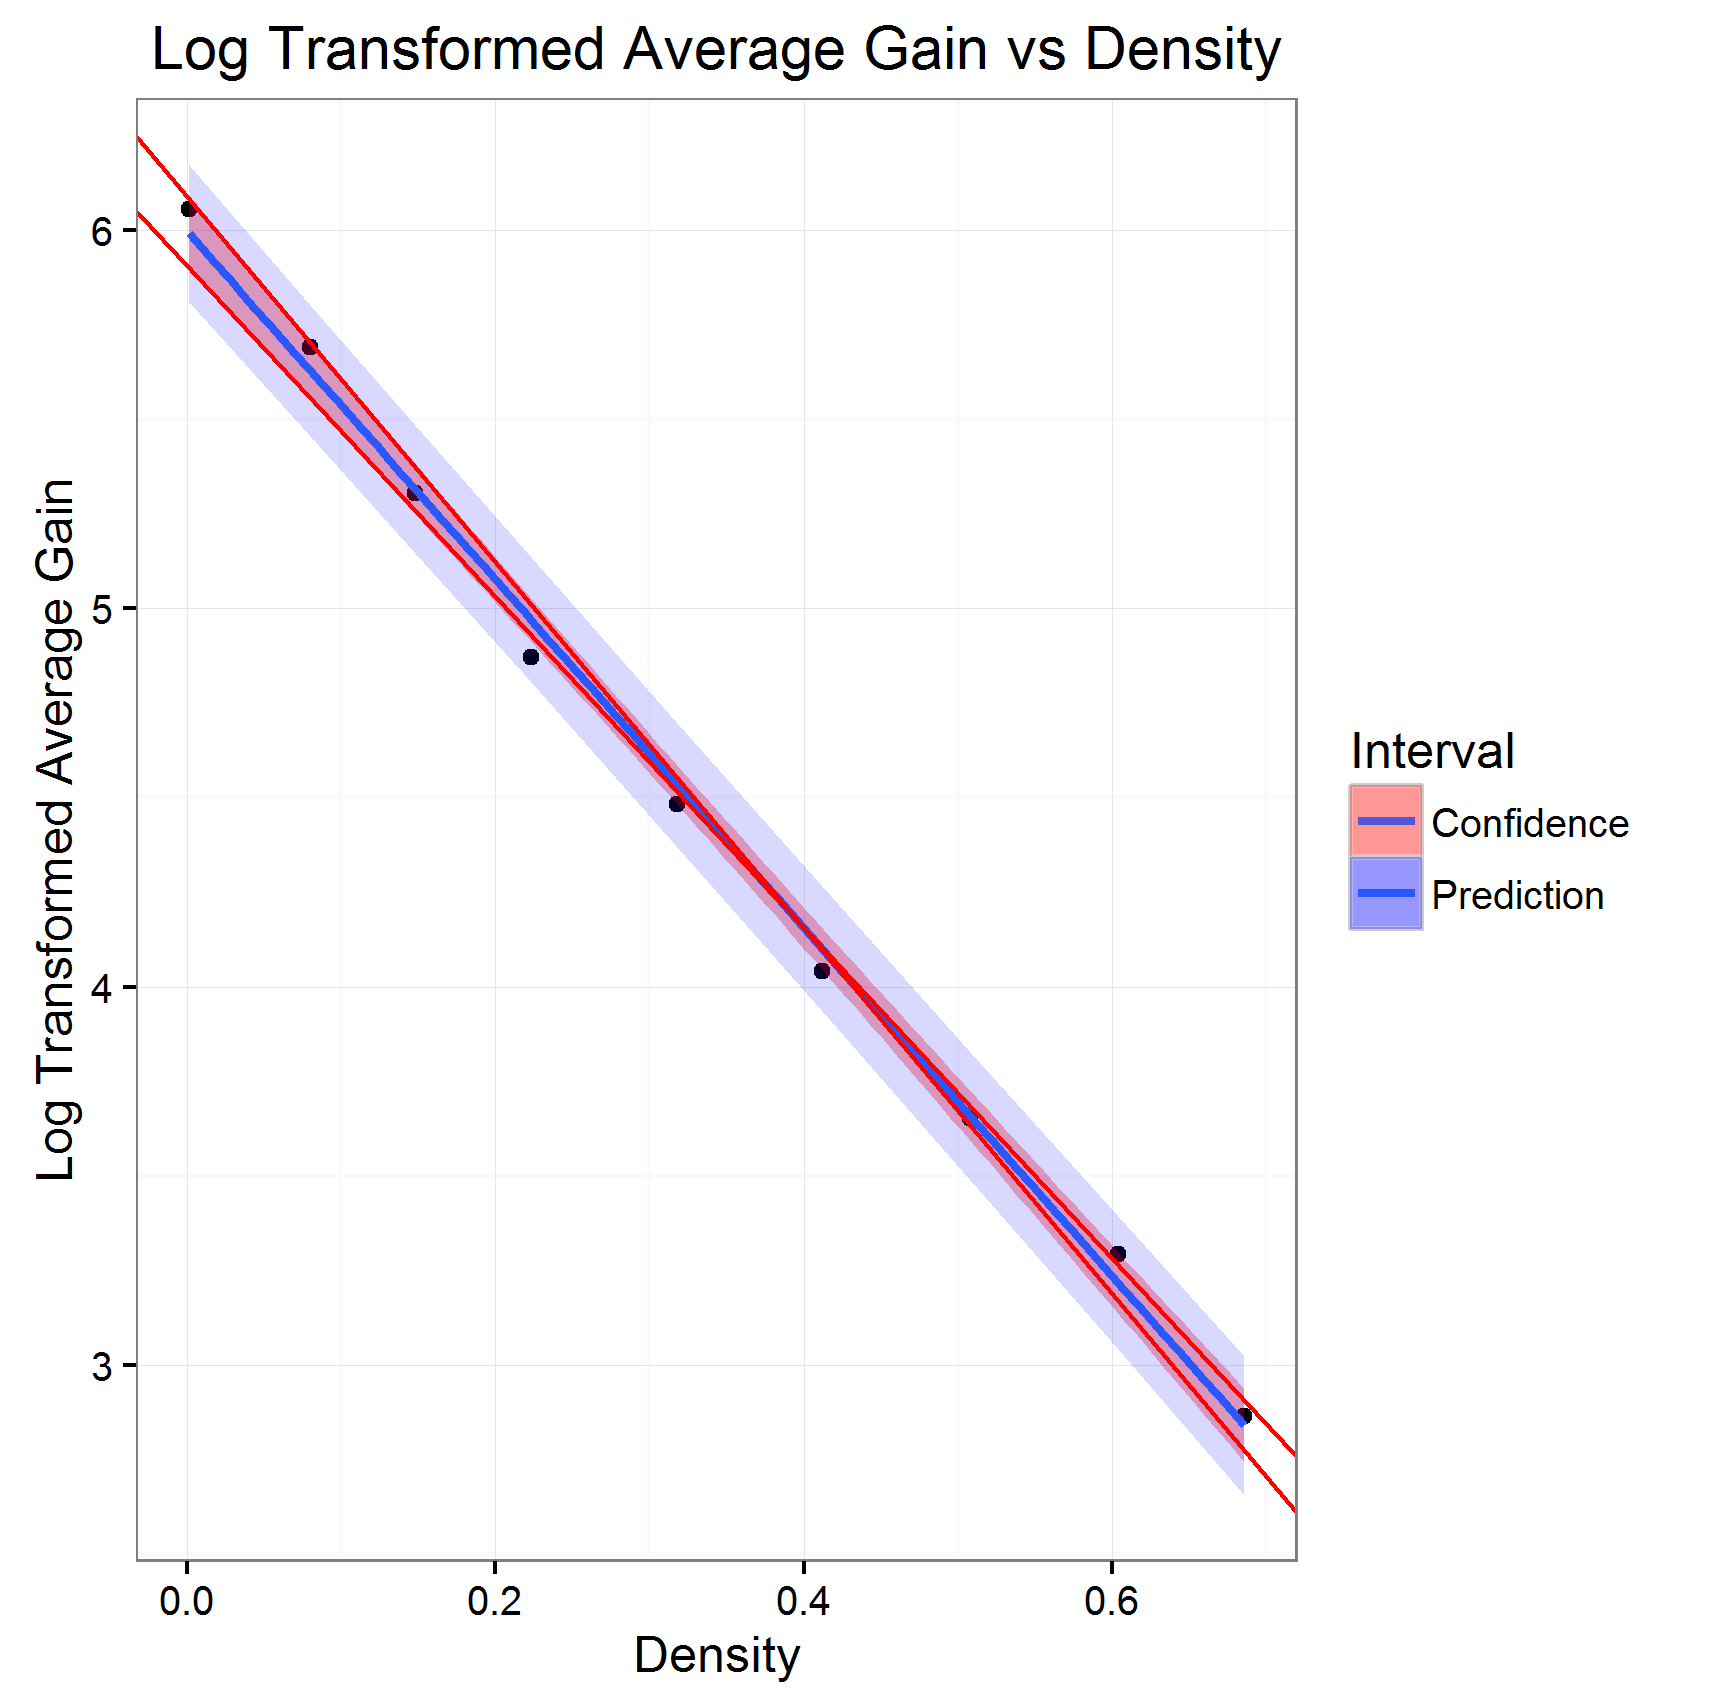
\includegraphics[scale=0.6]{logGainDensity.png}\end{center}

We ran the regression on the average of the log transformed gain values rather than on every individual point because we are dealing with data that are not independent. Since we have 10 observations from the same block, our linear model would be biased if we ran the regression on all the data points . This is because the linear model assumes measurements are taken independently. That is, if the true model is $Y_i=\beta_0 +\beta_1X_{i1}+\epsilon_i$, but a regression on all points would be $Y_i=\gamma_0+\gamma_1W_i$ where $W_i=X_i+\eta_i$. In this case, $Y_i$ is our prediction, $w_i$ is our observation where $X_i$ is observed with error, and $/beta$ is our true model. And with this model, we would have a bias of $\gamma_1=\beta_1\frac{var(x)}{var(x)var(\eta)}$. Therefore, we average the gain data with the same density to achieve independence. As a result, we run regression on only nine points with the formula $$\hat{X_i}=Q_i=\frac{1}{J}\sum_{j=1}^{J}W_{ij}$$ where $Q_i$ is our predicted value of $X$ and $J$ is our number of repeated measurements.

From this graph, we analyzed and plotted the residuals. Our residual plot only contains 9 data points, but each point is close enough to 0, indicating homoscedasticity, that we can conclude that a linear model is appropriate for fitting our data. This concurs with our initial assessment that the regression line closely matches the averaged data points.
\begin{center}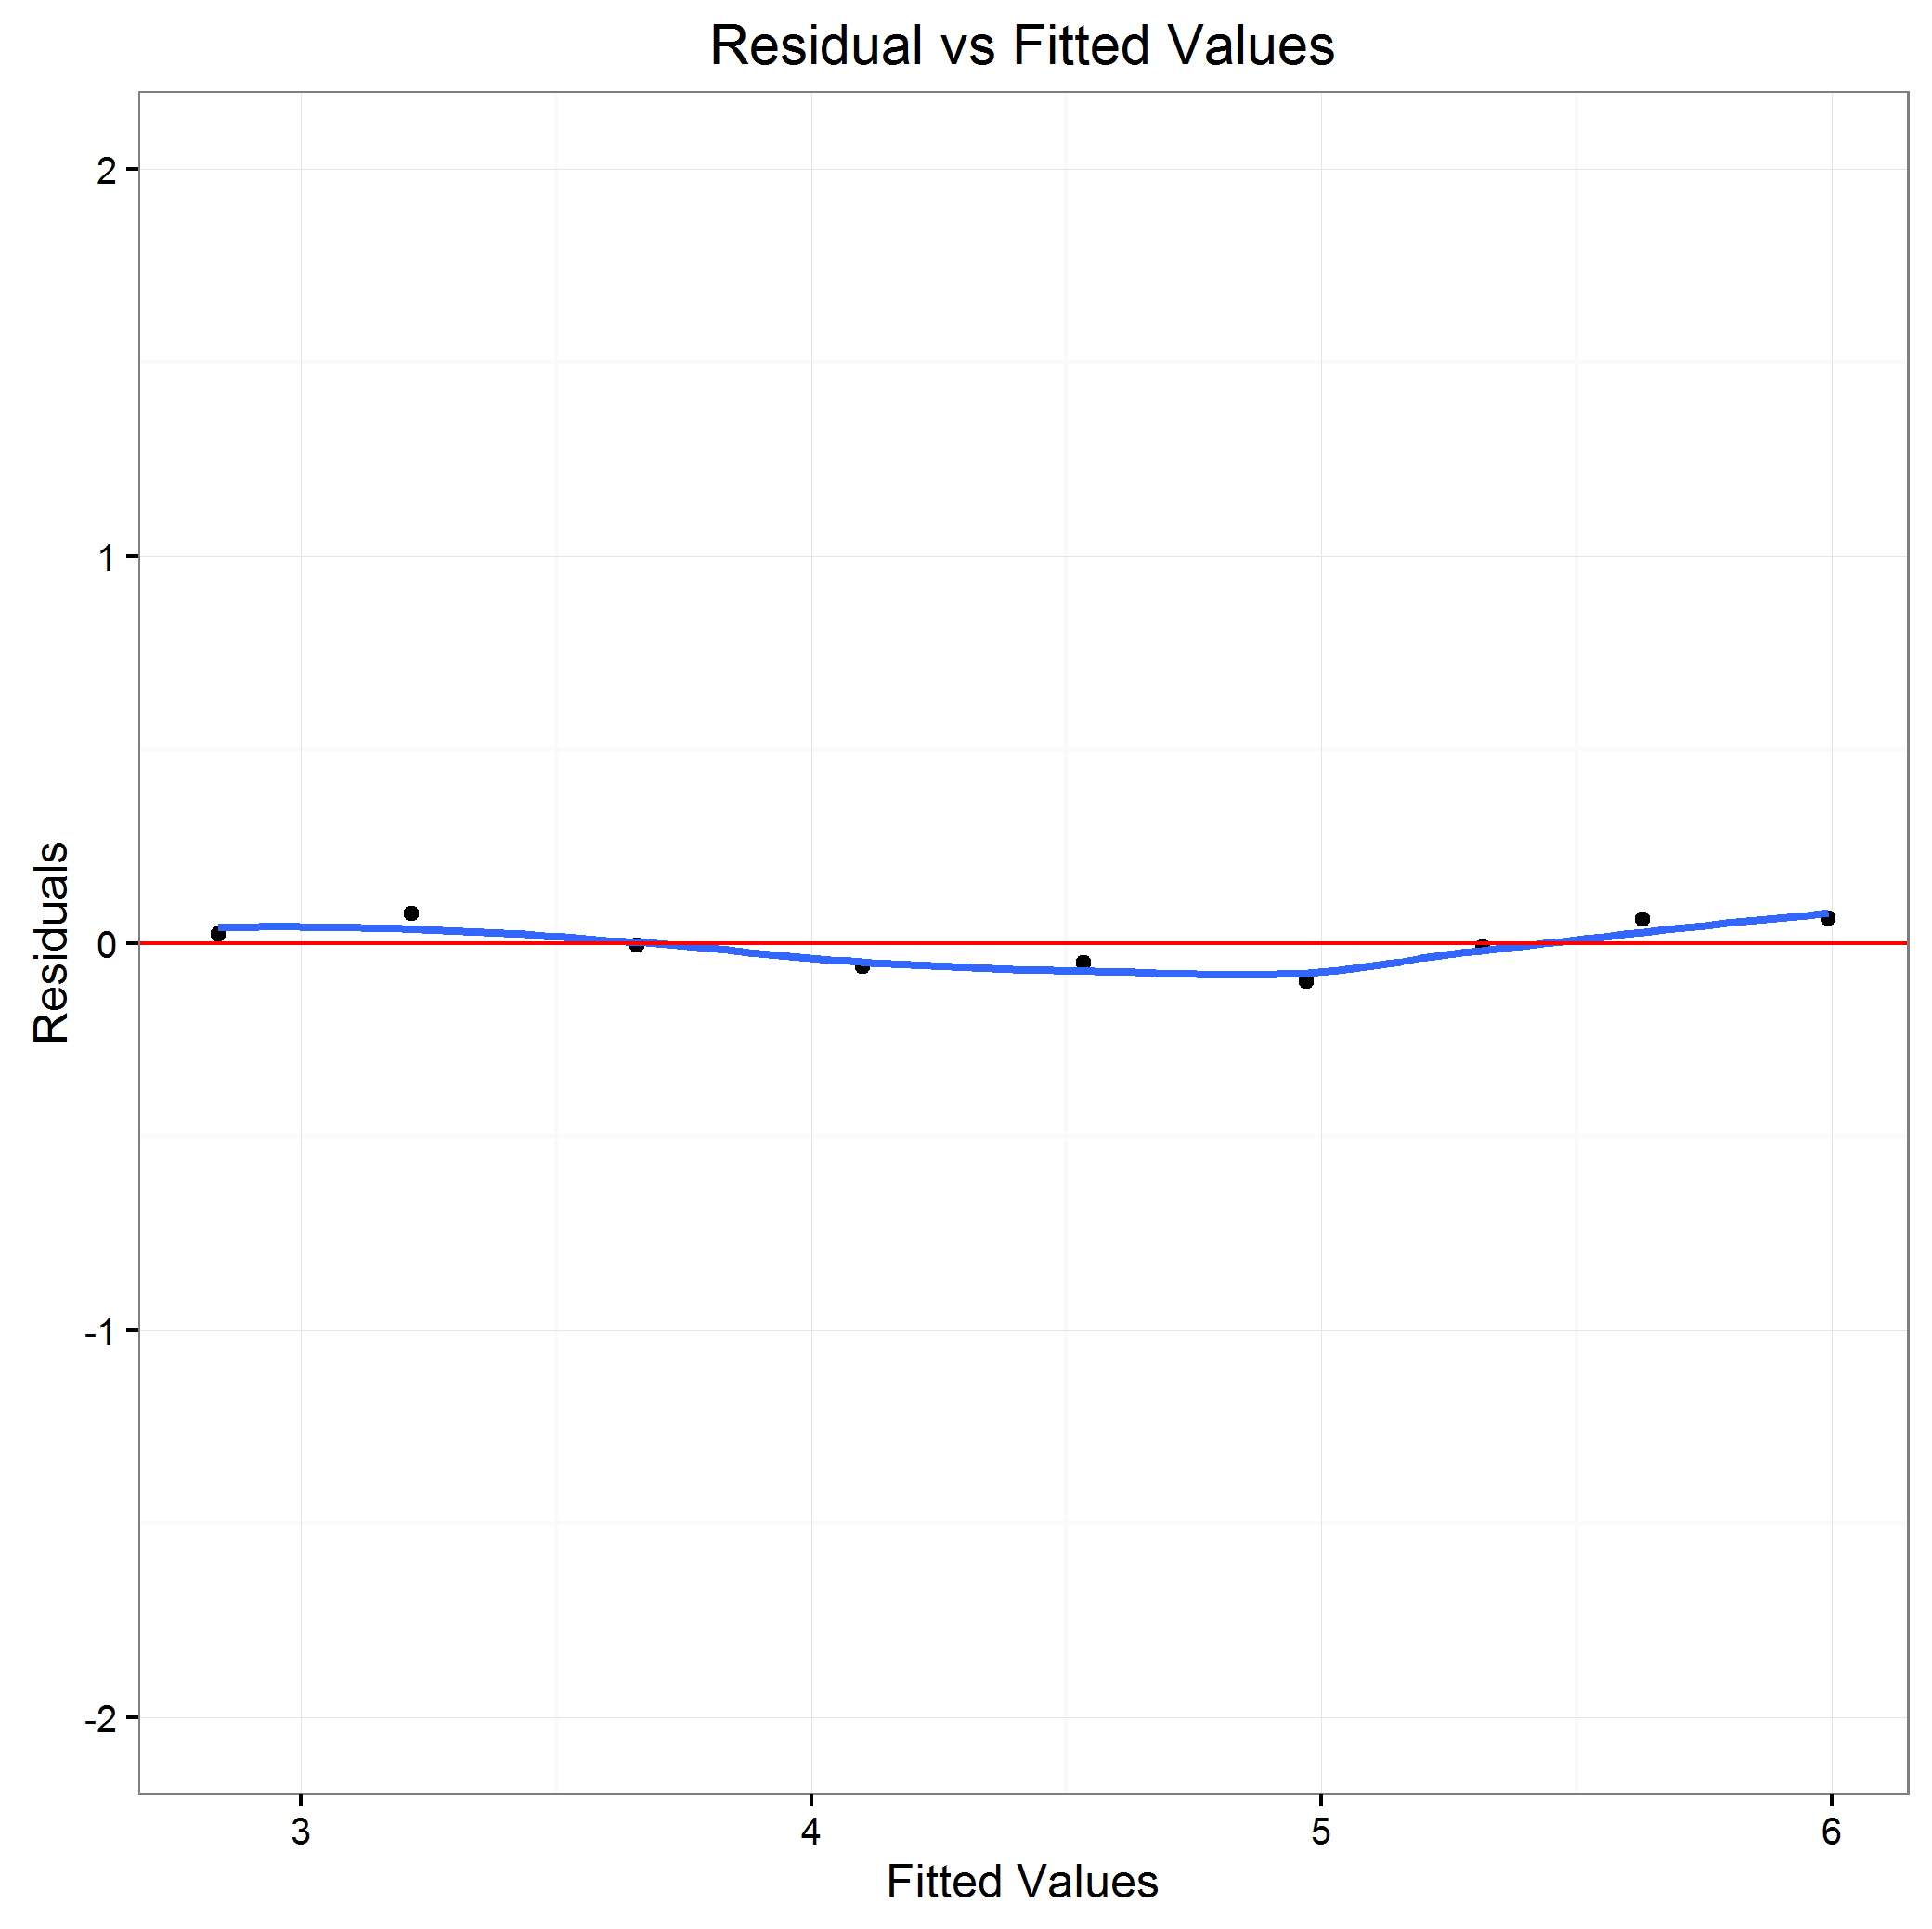
\includegraphics[scale=0.5]{residualsPlot.png}\end{center}

Another requirement of linear regressions is that the residuals should be normally distributed. To verify this, we made a QQ plot of the residuals, shown below. Because there are only 9 data points, it’s hard to say if the residuals are normal or not, but the dots approximately follow the normal line, indicating the residuals are relatively normal.
\begin{center}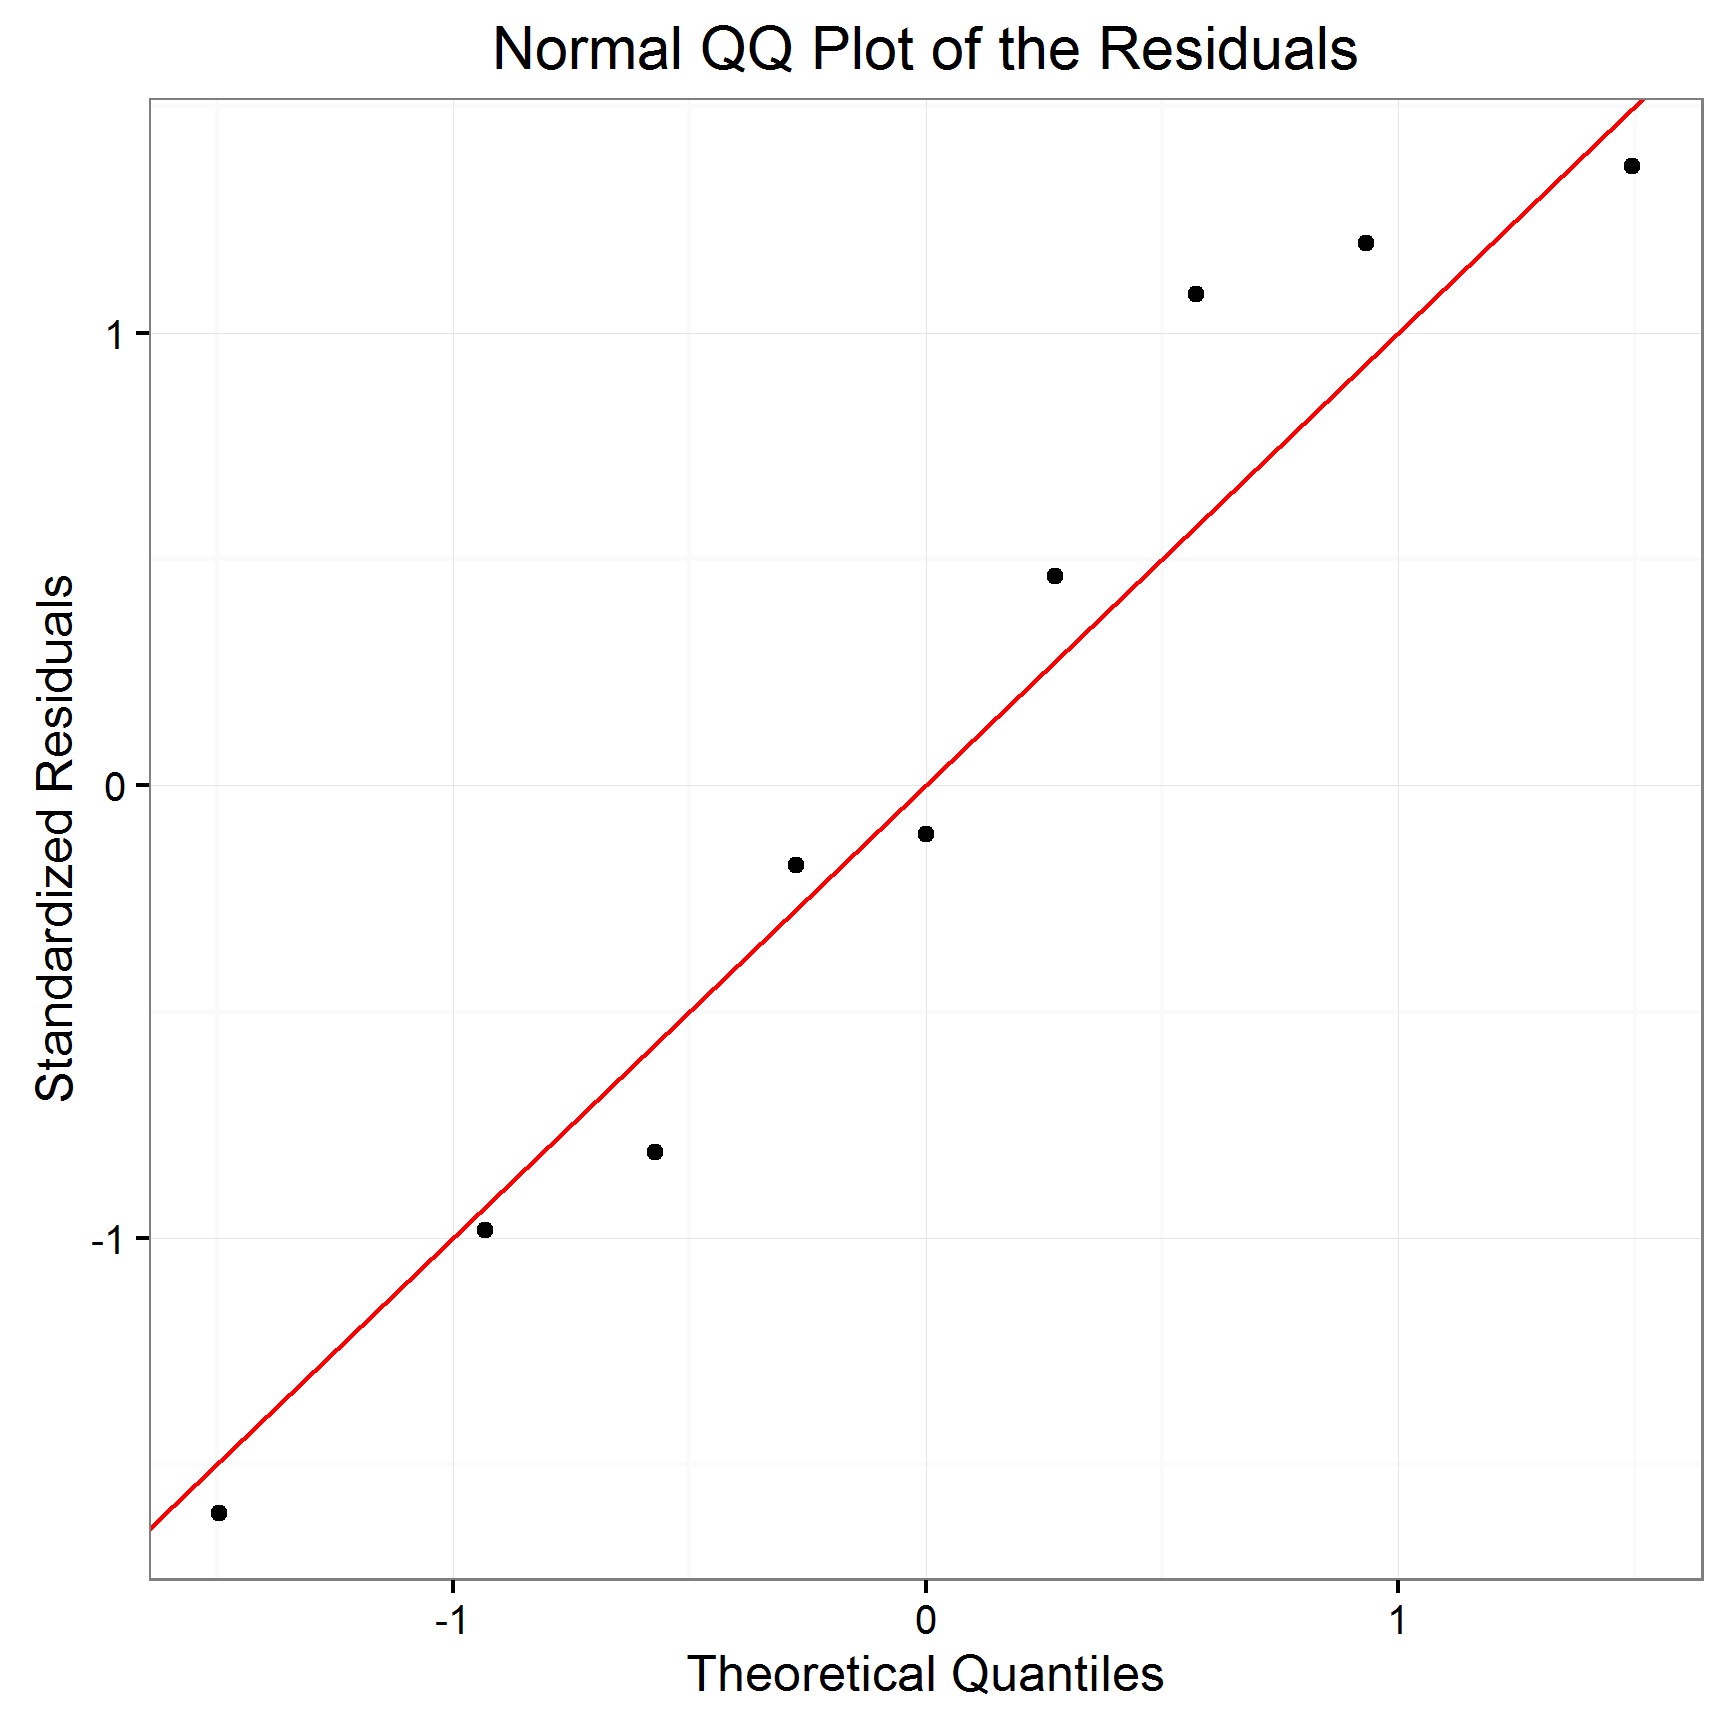
\includegraphics[scale=0.5]{qqPlotResiduals.png}\end{center}

\section*{Prediction}
Using this linear model of gain versus density, we plotted the predicted densities for gain values of 38.55 and 426.7. For a gain of 38.55, we predicted a density of $0.5088 g/cm^3$ with a 95\% confidence prediction interval of 0.4722 to $0.5455 g/cm^3$. The given density was $0.5080 g/cm^3$. Given a gain of 426.7, our model produces an expected density of $-0.01174 g/cm^3$ with a prediction interval of -0.05125 to $0.02778 g/cm^3$, compared to the given density of $0.0010 g/cm^3$. This prediction is evidently flawed, as density cannot be a negative number. One possible reason for this impossible density value is the small size of training data. This could be rectified by a larger training set.

\section*{Cross-validation}
To cross validate our linear model, we generated two other models based on the averaged data: one with the average gain for the $0.508 g/cm^3$ block removed, and the other with the $0.001 g/cm^3$ block removed. With these two models, we produced new density predictions for the gain of 38.55. Without the $0.508 g/cm^3$ data point, our model calculated density to a value of $0.5090 g/cm^3$, while eliminating the $0.001 g/cm^3$ block gave us a prediction of $0.5093 g/cm^3$. Compared with the first prediction value computed with no omitted data, both of these cross validation models appear to verify the robustness of our original model.

\section*{Conclusion}
From the residual vs. fitted values plot, it is clear that there are no major issues with the fit. The residuals are well within $\pm2$. The plot seems homoscedastic, but it is difficult to determine this since there are so few points. Additionally, since the quantile-quantile plot only has nine values, it is difficult to interpret.

If the densities of the polyethylene blocks do not contain accurate reports, then there will be error in the explanatory variable, which makes it necessary to take multiple observations. From this, the model now also takes into account the reliability of the measurements, and so becomes a biased estimator for the true linear model.

If the blocks of polyethylene were not measured randomly, then each gain reading’s error is not independent of each other, indicating that the gain error in each successive reading would be correlated to the block. This would result in a systematic bias, which is difficult to remove.

For a gain of 38.55, the model predicted a density of $5.089 g/cm^3$ with a lower bound of $0.4721 g/cm^3$ and an upper bound $0.5455 g/cm^3$. For a gain of 426.7, the model predicted a density of $-0.0117 g/cm^3$ with lower bound of $-0.0512 g/cm^3$ and an upper bound of  $0.0278 g/cm^3$. In our first cross-validation, the new model predicted $0.5090 g/cm^3$ for a gain of 38.55 , with upper bound $0.4673 g/cm^3$ and lower bound $0.5507 g/cm^3$. In the second cross-validation, our model predicted a density of $0.5093 g/cm^3$ for the same gain, with upper bound $0.472184 g/cm^3$ and lower bound $0.5464498 g/cm^3$. Overall, the procedure can accurately calibrate the snow gauge except in cases where the gain is large.

\section*{References}
\begin{enumerate}[1.]
\item Armstrong, R. L. (1976). The Application of Isotopic Profiling Snow Gauge Data to Avalanche Research. 606(76). Boulder, CO: Institute of Arctic and Alpine Research.
\item Bergman, J.  A. (1982). Two Standard Precipitation Gauges and the Gamma Transmission Snow Gauge: A Statistical Comparison. 358. Berkeley, CA: Pacific Southwest Forest and Range Experiment Station, Forest Service, U.S. Department of Agriculture.
\item Kattelmann, R. C., McGurk, B. J., Berg, N. H., Bergman, J. A, Baldwin, J.  A.\& Hannaford, M. A. (1983). The Isotope Profiling Snow Gauge: Twenty Years of Experience. 723(83). Berkeley, CA: Pacific Southwest Forest and Range Experiment Station, Forest Service, U.S. Department of Agriculture.
\end{enumerate}

\end{document}
